\section{Explorativer Teil: Automatisierung der Rechnungseinreichung der AXA Gesundheitsvorsorge}
\label{chap:experiment}

In diesem Kapitel wird ein Fallbeispiel erarbeitet, welches zeigen soll, ob künstliche Intelligenz mit kleinem Budget und wenigen Ressourcen zur Automatisierung von Geschäftsprozessen angewendet werden kann. 

Im folgenden wird eine Einführung in das Fallbeispiel gegeben und der relevante Prozess im Detail erläutert. Es werden Anforderungen definiert, welche erfüllt werden müssen, damit der relevante Prozessschritt und somit der gesamte Prozess automatisiert werden kann.

Das Vorgehen und die Methodik dieses explorativen Teil werden in einem eigenen Kapitel erläutert. Anhand dieses Vorgehens werden zwei für die Automatisierung des Prozesschrittes relevante Aspekte betrachtet. Zu diesen beiden Aspekten werden jeweils zwei Experimente durchgeführt, mit welchen die Machbarkeit der Automatisierung des Aspektes gezeigt werden soll.

Zu jedem Experiment werden die Ergebnisse diskutiert und, wo sinnvoll, mögliche Fehlerquellen analysiert. Verbesserungsvorschläge um Fehler zu minimieren werden im Kapitel \ref{chap:summary} vorgestellt.

% Innerhalb des weltweiten AXA Versicherungskonzern ist die Gesundheitsvorsorge ein in-House Startup innerhalb der AXA Schweiz. Es steht nur ein begrenztes Budget und begrenzte Ressourcen zur Verfügung. 

% In diesem Kapitel wird die Anwendbarkeit der künstlichen Intelligenz zur automatisierten Verarbeitung von eingereichten Rechnungen bei der AXA Gesundheitsvorsorge überprüft.

% Es wird erst ein Überblick über den Prozess gewährt, aus welchem anschliessend Aufgaben abgeleitet werden, welche mit Hilfe von künstlicher Intelligenz automatisiert werden sollen.

\subsection{Einführung in das Fallbeispiel}
In der Schweiz beliefen sich die Kosten für das Gesundheitswesen im Jahr 2015 auf 77.8 Milliarden Franken. Über 35\% dieser Kosten wurden durch die obligatorische Krankenversicherung gedeckt. Weitere knapp 7\% wurden von den Zusatzversicherungen übernommen. Die Krankenversicherer finanzierten also mit knapp 42\% einen beträchtlichen Teil des Gesundheitswesens in der Schweiz~\autocite{BfS2018}.

Die Kosten des Gesundheitswesen steigen stetig an, so weisen die Zahlen vom Jahr 2016 bereits Kosten von über 80 Milliarden Franken nach~\autocite{BfS2018}. Auch in den folgenden Jahren sollen die Kosten weiter steigen. \textcite{Kirchgassner2009} begründet diesen Anstieg unter anderem mit der Veränderung der Altersstruktur, dem steigenden Wohlstand sowie den neuen Möglichkeiten in der Diagnose und Behandlung durch technischen Fortschritt.

Die Kosten, welche die Krankenversicherer tragen, werden mit einem von zwei Systemen, \textit{Tiers payant} oder \textit{Tiers garant}, vergütet (vgl. Tabelle \ref{tiers}~\autocite{EDI2017}. 

\begin{wraptable}{l}{0.53\textwidth}
    \renewcommand{\arraystretch}{1.25}
    \setlength{\tabcolsep}{5pt}
    \caption{Vergütungsmodelle bei den schweizer Krankenversicherern}
    \label{tiers}
    \begin{tabular}{| p{0.15\textwidth} | p{0.32\textwidth} |}
        \hline
         Tiers payant & Kosten werden vom Leistungserbringer direkt dem Krankenversicherer in Rechnung gestellt. \\
        \hline
         Tiers garant & Kosten werden vom Leistungserbringer dem Patienten in Rechnung gestellt, welcher die Rechnung dem Krankenversicherer zur Rückvergütung weiterleitet. \\
        \hline
    \end{tabular}
\end{wraptable}

Beim System Tiers payant belastet der Leistungserbringer (bspw. Arzt oder Apotheke) die Kosten direkt dem Krankenversicherer. Dies geschieht, indem der Patient mit seiner Versichertenkarte bezahlt. Anhand dieser Versichertenkarte, welche vom Krankenversicherer ausgestellt wird, können Deckungen für den Patienten überprüft sowie die Rechnung direkt an den Krankenversicherer übermittelt werden. In diesem Fall wird die Rechnung bereits in digitaler, strukturierter Form übermittelt~\autocite{EDI2017}. 

Werden Kosten, welche über Tiers payant abgerechnet wurden, nicht vom Krankenversicherer getragen, weil beispielsweise ein Selbstbehalt vereinbart wurde, die Franchise noch nicht aufgebraucht ist oder der Patient für diese Behandlung gar nicht versichert ist, verrechnet der Krankenversicherer die Kosten dem Patienten weiter \autocite{EDI2017}.

Das System Tiers payant wird häufig in Apotheken, beim Kauf von Medikamenten mit oder ohne ärztlichem Rezept, sowie bei allen stationären Behandlungen, gemäss Art. 42 Abs. 2 KVG, verwendet \autocite{EDI2017}.

Die Verarbeitung von Rechnungen, welche über das System Tiers payant abgerechnet werden, kann der Krankenversicherer, aufgrund der digitalen, strukturierten Daten, automatisiert gestalten~\autocite{BAG2016}.

Im Fall von Tiers garant stellt der Leistungserbringer die Rechnung direkt dem Patienten aus, welcher diese dann seinem Krankenversicherer zur Rückerstattung weiterleitet. Die Rechnung kann bei allen Krankenversicherern per Post und bei den meisten auch digital, im Kundenportal oder in der App, eingereicht werden \autocite{EDI2017}.

Rechnungen, welche per Post oder digital beim Krankenversicherer zur Rückvergütung eingehen, erreichen diesen in verschiedenen Formen und unterschiedlichster Qualität. 

Während einige Rechnungen nach dem TARMED Standard für Rückforderungsbelege strukturiert sind, sind andere formlos. Die Bandbreite dieser Formlosen Rechnungen ist gross: Von handgeschriebenen Rechnungen eines örtlichen Leistungserbringer bis hin zu strukturierten Rechnungen von Fitnessketten.

Bei der Einreichung per Post kann die Qualität durch Kaffee-Flecken, Verbleichung der Belege oder sonstige Beeinträchtigungen gemindert werden, der Krankenversicherer kann aber einiges dazu beitragen die Rechnung in hoher Qualität einzulesen. So kann er beispielsweise hochauflösende Scanner und eine optimale Beleuchtung einsetzen.

Problematischer sind Rechnungen, welche von Kund/-innen digital, sprich als Foto , an den Krankenversicherer übermittelt werden. Wird ein Foto einer Rechnung über das Kundenportal eingereicht, so hat der Krankenversicherer nur noch sehr wenig Einfluss auf die Qualität der Aufnahme. Schlechte Belichtung, kleine Auflösung und abgeschnittene Rechnungen sind nur wenige der Probleme, mit welchen der Krankenversicherer zu kämpfen hat.

Egal wie und in welcher Qualität eine Rechnung einen Krankenversicherer erreicht hat, muss dieser die Rechnung in eine elektronische, strukturierte Form bringen, damit diese dann durch ein Regelwerk verarbeitet werden kann. Dieser Vorgang wird durch verschiedenste Techniken aus den Bereich der Texterkennung und der Informationsextraktion ermöglicht. Als Texterkennung oder auch Optical Character Recongition (kurz OCR) wird ein Vorgang bezeichnet, bei welchem Handschrift oder Druckbuchstaben in eine Form gebracht werden, welche von Maschinen verstanden und bearbeitet werden kann~\autocite{Xue2014}. Unter dem Begriff Informationsextraktion oder Information extraction (kurz IE) wird der Prozess verstanden, bei welchem relevante Fakten aus einem Text gewonnen werden~\autocite{Piskorski2012}.

% \todo[inline, color=green]{Wie macht das die Post? Postfinance? Dort ist das Problem vermutlich etwas einfacher aber Lösungen gibt es schon länger?}

% Viele Krankenkassen haben diese Technologien bereits im Einsatz. Auch gibt es diverse Anbieter, wie beispielsweise die Tessi document solutions (Switzerland) GmbH oder die Cent Systems AG, welche diese Technologien oder gar umfangreiche Services in diesem Bereich anbieten. Die Erfahrung mit diesen Technologien und Providern bei der AXA Ein grosser Teil der Rechnungen muss aber, aus verschiedenen Gründen, nach wie vor manuell bearbeitet werden \todo{Quelle für manuelle arbeiten}. Dies beinhaltet sowohl die Nachbearbeitung nach der elektronischen Indexierung als auch die komplett manuelle Indexierung\todo{CITE}. 
% Die CSS Krankenkasse beschäftigt beispielsweise rund 200 Personen für diese manuelle Indexierung. Bei der Assura sind es rund 500 Personen \todo{Quelle für die Anzahl personen}.

% Im Jahr 2016 wiesen die Grundversicherer einen durchschnittlichen Verwaltungskostensatz von 4.7\% aus. Dies bedeutet  Ein guter Verwaltungskostensatz konnte die CSS Kranken-Versicherung AG im Jahr 2017 ausweisen weist im Jahr Die Indexierung dieser Rechnungen ist einer der Faktoren, welche auf die hohen Verwaltungskosten der Krankenversicherer schlägt.

Die AXA, eine internationale Versicherungsgesellschaft, sieht sich, genau wie alle anderen Krankenversicherer, ebenfalls vor der Herausforderung der Indexierung von Rechnungen. Im Jahr 2017 lancierte die AXA eine Zusatzversicherung in der Gesundheitsvorsorge im Schweizer Markt. Neben der Zusatzversicherungen selbst bietet die AXA ihren Kunden einen Rechnungs-Weiterleitungs-Service an. Das bedeutet, alle Rechnungen können der AXA gesendet werden, auch wenn diese die Grundversicherung betreffen. Rechnungen beziehungsweise Rechnungspositionen, welche die Zusatzversicherung betreffen, werden von der AXA vergütet. Rechnungspositionen, welche die Grundversicherung betreffen, werden zur Vergütung an den Grundversicherer weitergeleitet \autocite{Finanzen.ch2017}.

Gemäss einem Beitrag auf \textcite{Finanzen.ch2017} ist es das Ziel der AXA, bis im Jahr 2020 insgesamt 100'000 Kunden für die Gesundheitsvorsorge zu gewinnen. Aus dem Geschäftsbericht der CSS Gruppe für das Jahr 2017 geht hervor, dass für knapp 1.7 Millionen Kunden 16 Millionen Rechnungen geprüft wurden~\autocite{CSSGruppe2018}. Werden die durchschnittlich 9.5 Rechnungen pro Kunde der CSS Gruppe auf die Zielgrösse 100'000 Kunden der AXA hochgerechnet, so muss die AXA im Jahr 2020 knapp 1 Million Rechnungen prüfen. Damit diese Menge an Rechnungen effizient verarbeitet werden kann, ist es für die AXA wichtig, den Prozess der Indexierung möglichst automatisiert zu gestalten.

Um die Verwaltungskosten der Zusatzversicherung aufzuzeigen wird wiederum der Ge\-schäfts\-be\-richt der CSS Gruppe für das Jahr 2017 herangezogen. Der Kostensatz, welcher den Anteil der Gemeinkosten am Umsatz misst, betrug für die Grundversicherung lediglich 4\%. Im Geschäftsbereich der Zusatzverischerungen liegt dieser Kostensatz allerdings viel höher, nämlich bei 21\%~\autocite{CSSGruppe2018}. Welcher Anteil an diesen Kosten nun der Prüfung respektive der Indexierung eingehender Rechnungen zuzuschreiben ist, bleibt ein Betriebsgeheimnis. Da die Rechnungen, welche die Zusatzversicherungen betreffen, aufgrund der unterschiedlichen Leistungserbringer (Alternativmedizin, Fitness, Sportverein) viel diverser sind als jene die die Grundversicherung (meist ausgestellt durch Ärzte und Spitäler nach TARMED standard) betreffen, liegt die Vermutung nahe, dass im Bereich der Zusatzversicherung ein hoher Anteil der Verwaltungskosten der Rechnungsprüfung zugeschrieben werden kann.

Die AXA profitiert aber bei einer automatisierten Indexierung von Rechnungen nicht nur von einer Kostensenkung sondern kann damit auch einen Vorteil für Ihre Kunden generieren: Die Kunden erhalten durch die automatisierte Verarbeitung der eingereichten Rechnungen viel schneller das geforderte Geld.

%Rechnungen, egal ob diese von der AXA selbst bezahlt oder an den Grundversicherer weitergeleitet werden, müssen indexiert werden um verarbeitet werden zu können. Die Indexierung wird aktuell von einem externen Provider übernommen und ist eine \todo[color=yellow]{erläutern}Blackbox. Es ist allerdings bekannt, dass ein grosser Teil der Arbeiten, nach einem automatisierten OCR Schritt, manuell gemacht werden. Die aktuelle Indexierung birgt folgende zwei Probleme:

%\todo[inline, color=igloo]{Hinweis: Ich weiss, ist eine provokative Frage. Aber ich frage mich, ob es Sinn macht, dies so zu erwähnen, weil daraus entstehen Fragen -> Warum dieser Provider, wenn nicht klar ist, was er macht? Oder warum wird nicht das Know-how akquiriert?}

%\todo[inline, color=igloo]{Frage: Warum müssen die Rechnungen indexiert werden? Bitte kurz erklären, warum dies Unternehmen machen. }

\subsubsection{Aktueller Prozess der Rechnungseinreichung}

Der Prozess der Rechnungseinreichung und -verarbeitung (vgl. Abbildung \ref{prozessaxa}) der AXA kann aufgrund der zwei im vorherigen Kapitel erwähnten Ereignisse angestossen werden: Der Kunde kann entweder digital oder per Post eine Rechnung einreichen. 

\begin{figure}[h]
    \captionsetup{width=.8\linewidth}
    \caption{Prozess der Rechnungseinreichung und -verarbeitung der AXA Gesundheitsvorsorge. Vom Kunden per Post oder über das Kundenportal eingereichte Rechnungen durchlaufen mehrere Prozessschritte in Verantwortung unterschiedlicher Organisationen.}
    \label{prozessaxa}
    \centering
    \vspace{0.2cm}
    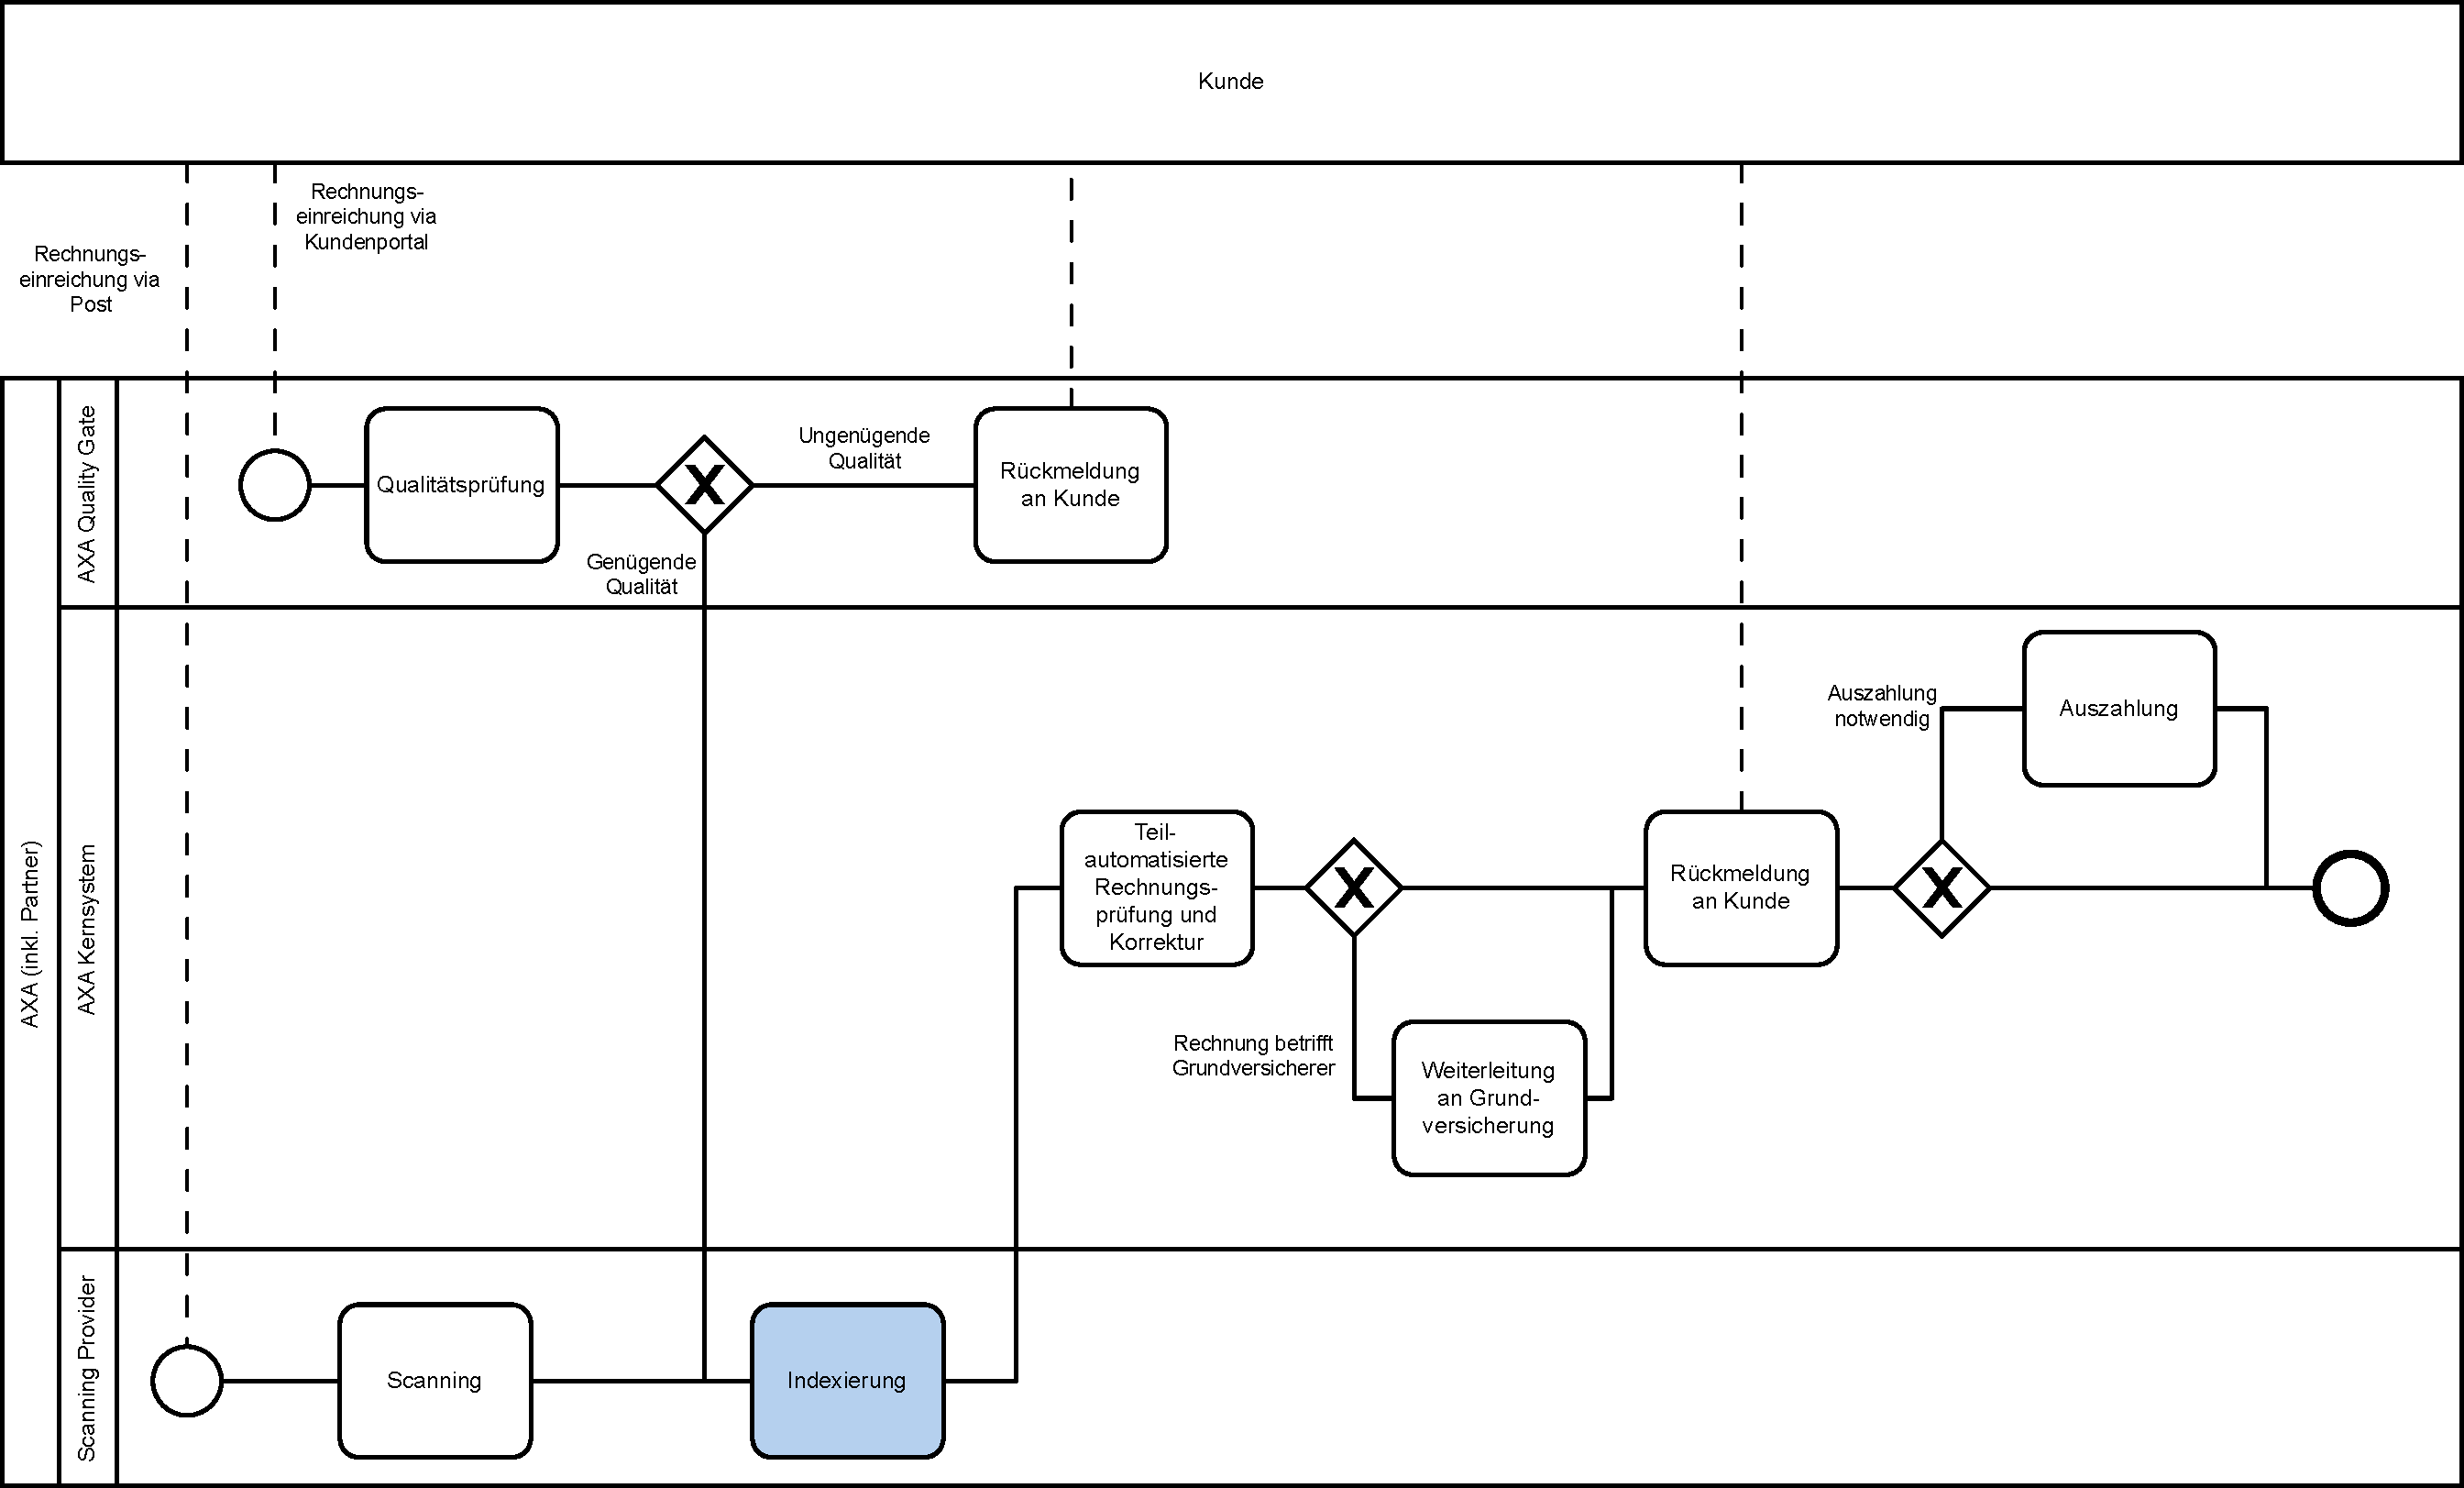
\includegraphics[width=\textwidth]{graphics/rechnungseinreichung-bpmn.pdf}
\end{figure}

\todo[inline]{Im BPMN Diagramm SVG export fehlen die Pfeile...}

Im Kundenportal hat der Kunde die Möglichkeit eine Rechnung hochzuladen. Dabei kann er entweder ein Dokument auf seinem Endgerät wählen oder die Kamera seines Geräts nutzen, um eine Rechnung zu fotografieren.

Nach erfolgreichem Hochladen der Rechnung im Kundenportal durchläuft diese eine erste manuelle Qualitätsprüfung. Diese Qualitätsprüfung wurde eingeführt, da hochgeladene Rechnung teilweise ungenügende Qualität vorweisen. Entspricht die Rechnung nicht den Qualitätsanforderungen oder fehlt eine Seite oder eine ärztliche Verordnung, so wird der Kunde gebeten, die vollständige Rechnung erneut hochzuladen.

Nach erfolgreicher Qualitätsprüfung wird die Rechnung an den Scanning und Indexierungsdienstleister der AXA weitergeleitet.

Entscheidet sich der Kunde für die Einreichung per Post, so wird sein Brief direkt an den Scanning und Indexierungsdienstleister der AXA weitergeleitet. Dieser Dienstleister scannt die weitergeleitete Rechnung ein.

Nach beiden dieser Einstiegspunkten in den Prozess indexiert nun der Scanning und Indexierungsdienstleister die eingereichte Rechnung. Dieser Aufgabenschritt erfolgt teilweise automatisiert und teilweise manuell. Wie genau die Indexierung abläuft ist nicht bekannt. Der genaue Ablauf dieser eingekauften Dienstleistung wird als Geschäftsgeheimnis gewahrt.

Nach der Indexierung werden die Scans sowie das strukturierte Resultat der Indexierung elektronisch an das Kernsystem der AXA Gesundheitsvorsorge übermittelt. Dieses Kern\-system verarbeitet die eingegangenen Rechnungen aufgrund eines Regelwerks. Kann die Rechnung nicht verarbeitet werden, weil diese nicht korrekt Indexiert wurde oder Informationen fehlen, muss eine FachspezialistIn eingreifen. Nach allfälligen Rückfragen und Korrekturen durch die FachspezialistIn wird die Rechnung verarbeitet. 

Nach der Erfolgreichen Verarbeitung der Rechnung wird der Kunde elektronisch informiert, ob die beanspruchten Leistungen versichert sind und ob eine Rückvergütung ausbezahlt wird.

Hat der Kunde die AXA bevollmächtigt, so wird die Rechnung in gewissen Fällen, je nach Rechnungspositionen, automatisiert an die Grundversicherung des Kunden weitergeleitet.

Ziel der AXA Gesundheitsvorsorge ist es, diesen Prozess für eingereichte Rechnungen, welche Fitnesscenter und Optiker betreffen, vollständig zu automatisieren. Dabei gibt es in diversen Bereichen Herausforderungen, welche aktuell angegangen werden. Diese Arbeit hat zum Ziel, die Herausforderungen im Bereich der Indexierung anzugehen. Es wird untersucht, ob die Anwendung künstlicher Intelligenz eine Automatisierung der Indexierung ermöglichen kann.

Ausgangslage für den Arbeitsschritt der Indexierung ist eine digitalisierte Rechnung. Ziel der Indexierung ist es, aus dieser Rechnung strukturierte Informationen zu gewinnen und an das Kernsystem der AXA zu übermittelt. In dieser Arbeit wird die Extraktion dieser strukturierten Daten aus den digitalisierten Rechnungen mit Hilfe künstlicher Intelligenz behandelt. Das Übermitteln der strukturierten Informationen an das Kernsystem ist bereits gelöst und aus diesem Grund kein Teil der Untersuchungen dieser Arbeit.

% Um den Umfang dieser Analyse einzugrenzen, wird der Fokus auf Rechnungen von Optikern, Fitnesscentern und Sportvereinen gelegt. Diese Rechnungen machen 23\% der eingereichten Rechnungen aus und sind Versicherungstechnisch relativ einfach handzuhaben.

% optiker 2660 -> 
% fitness 2055
% sportsclub 847
% =subtotla 5562
% other 18881
% =total 24443


\subsection{Anforderungen}

Um Rechnungen von Fitnesscenter und Optikern automatisiert verarbeiten zu können, müssen diese Rechnungen als solche klassifiziert und die notwendigen Informationen, welche nachfolgend genauer spezifiziert werden, extrahiert werden.

Um eine Rechnung eines Optikers zu verarbeiten, sind folgende Informationen relevant:

\begin{itemize}
    \item \textbf{Leistungsbezüger}
    
    Es muss ermittelt werden, für wen die Rechnung ausgestellt wurde. Anhand dieser Information wird geprüft, ob und wie diese Person bei der AXA versichert ist. Auch wird damit geprüft, dass der maximal versicherte Betrag noch nicht ausgeschöpft ist.
    
    Ist der Leistungsbezüger minderjährig, so wird ein gewisser Betrag von der Grundversicherung übernommen. In diesem Fall wird dieser Betrag von der Rückvergütung der AXA abgezogen und die Rechnung an die Grundversicherung weitergeleitet.
    
    \item \textbf{Totalbetrag der Rechnung (inkl. Währung)}
    
    Dieser Betrag bildet die Grundlage zur Berechnung der geschuldeten Leistung an den Kunden. 
    
    Einzelne Rechnungspositionen sind für Rechnungen von Optikern nicht relevant.
    
    \item \textbf{Hinweis auf eine ärztliche Verordnung}
    
    Besteht eine ärztliche Verordnung, ist ein gewisser Betrag bei der Grundversicherung versichert. In diesem Fall wird dieser Betrag von der Rückvergütung der AXA abgezogen und die Rechnung an die Grundversicherung weitergeleitet.
\end{itemize}

%\paragraph{
%    \textbf{Relevante Attribute einer Rechnung für einen Sportverein}
%}

%Eine Rechnung eines Sportvereins wird bei der AXA Anhand folgender Attribute beurteilt:

%\begin{itemize}
%    \item \textbf{Leistungsbezüger}
%    
%    Es muss ermittelt werden, für wen die Rechnung ausgestellt wurde. Anhand dieser Information wird geprüft ob und wie diese Person bei der AXA Versichert ist. Auch wird damit geprüft, dass der maximal versicherte Betrag noch nicht ausgeschöpft ist.
%    \item \textbf{Totalbetrag der Rechnung (inkl. Währung):}
%    
%    Dieser Betrag bildet die Grundlage zur Berechung des geschuldeten Betrages. 
%    
%    Einzelne Rechnungspoisition sind für Rechnungen eines Sportvereins nicht relevant.
%    \item \textbf{Sportart}
%    
%    Die AXA anerkennt alle olympischen Sportarten. Das bedeutet, gewisse Sportarten sind nicht versichert. Es muss also die Sportart ermittelt werden, um die Versicherungsdeckung zu prüfen.
%\end{itemize}

Folgende Informationen sind notwendig, um eine Rechnung für ein Fitness-Abo zu verarbeiten:

\begin{itemize}
    \item \textbf{Leistungsbezüger}
    
    Es muss ermittelt werden, für wen die Rechnung ausgestellt wurde. Anhand dieser Information wird geprüft ob und wie diese Person bei der AXA versichert ist. Auch wird damit geprüft, dass der maximal versicherte Betrag noch nicht ausgeschöpft ist.
    \item \textbf{Totalbetrag der Rechnung (inkl. Währung):}
    
    Dieser Betrag bildet die Grundlage zur Berechnung der geschuldeten Leistung an den Kunden. 
    
    Einzelne Rechnungspositionen sind für Rechnungen von Optikern nicht relevant.
    \item \textbf{Fitnesscenter (Leistungserbringer)}
    
    Die AXA anerkennt alle Fitnesscenter mit dem Label Qualitop von Qualicert oder mit einer Bewertung von mindestens 3 Sternen bei Fitnessguide.
\end{itemize}

Anhand dieser Informationen können Rechnungen automatisiert verarbeitet werden. Es ist wichtig, dass diese Informationen korrekt extrahiert werden, denn durch die Automatisierung entfällt jegliche manuelle Prüfung. Fehler würden, wenn überhaupt, erst dem Kunden auffallen. 

\todo[inline]{Sollen hier bereits hard requirements (e.g. wieviele Rechnungen dürfen falsch indexiert werden) aufgestellt werden?}

\subsection{Vorgehen und Methodik}

Wie in den Anforderungen an die Indexierung bereits angemerkt, müssen zwei Teilschritte, die Klassifizierung und die Extraktion von Informationen, analysiert werden. Dabei kommt ein explorativer Ansatz zur Anwendung. Für beide Teilschritte wird je ein separates Experiment durchgeführt. Der Ablauf der Experimente ist dabei identisch. 

Für beide Experimente werden zuerst Testdaten aus dem System der AXA extrahiert und aufbereitet. Für die beiden Experimente werden jeweils eine oder mehrere künstliche Intelligenzen geschaffen. Die Resultate der beiden Experimente werden jeweils unabhängig voneinander diskutiert.

Aus den Diskussionen der beiden Experimente werden Schlussfolgerungen für die Anwendbarkeit der künstlichen Intelligenz zur Indexierung von Rechnungen abgeleitet. Neben dem Erfolg der Experimente werden dabei auch das Potential der gewählten Ansätze sowie mögliche weitere Ansätze diskutiert.



